%!TEX encoding=UTF-8 Unicode
\chapter{Memory Performance Analysis}

The results of our case study (\chap{perf}) showed that traditional performance analysis tools can help identify memory related performance issues.
Yet they are not able to tell precisely where, in terms of data structures, the issue occurs.
Thus it is still required to analyze the code manually.
As memory is often a performance bottleneck, several tools where developed to analyze performance in regards of the memory.

This chapter discuss memory analysis tools, first we present the specificities of recent memory subsystems and the usual mistakes that can generate performances drop in \sect{archi}.
Then we present existing memory performance analysis tools and discuss their limitation in \sect{mem-tools}.
Finally we describe what would be in idealistic memory performance analysis tool \sect{mem-cncl}.

\section{Architectural considerations}
\label{sec:archi}

Since a few decades, processor frequency increased significantly more than memory frequencies, resulting in a considerable gap between these two resources.
Retrieving one piece of data cost around $100$ \gls{CPU} cycles~\cite{Drepper07What}.
To mitigate this issue, the \glspl{CPU} embed several small and fast memory caches.
One access to the fastest cache usually cost about $10$ \gls{CPU} cycles.
These caches are organized hierarchically thus the time required to access a piece of data depends on the cache on which it is present.
Moreover several mechanisms where designed to guess which data should be in the cache.
As a result, a developer seeking for performances must consider the architecture of these caches and the way the work to benefit from them.

\begin{figure}[htb]
    \centering
    %!TEX encoding=UTF-8 Unicode
%Palette GnBu 5 col + white
\definecolor{ColPU}{HTML}{FFFFFF}
\definecolor{ColCore}{HTML}{F0F9E8}
\definecolor{ColL1}{HTML}{BAE4BC}
\definecolor{ColL2}{HTML}{7BCCC4}
\definecolor{ColL3}{HTML}{43A2CA}
\definecolor{ColM}{HTML}{0868AC}
\definecolor{ColS}{HTML}{FFFFFF}

\pgfdeclarelayer{bg}
\pgfdeclarelayer{bbg}
\pgfdeclarelayer{bbbg}
\pgfsetlayers{bbbg,bbg,bg,main}


\tikzset{
    box/.style={
        shape=rectangle,
        text centered,
        draw,
    },
    pics/core/.style args={#1#2#3#4}{
        % Args: #1: nb PU, #2 core id, #3 direction: + or -
        code={
            \pgfmathtruncatemacro{\pmin}{#1*#2}
            \pgfmathtruncatemacro{\pmax}{\pmin+#1-1}
            %PUs
            \foreach \pu in {\pmin,...,\pmax}{
                \pgfmathtruncatemacro{\pstep}{\pu-\pmin}
                \node[box,fill=ColPU] (PU-\pu)at (0,#3.7*\pstep) {PU\#\pu};
            }
            %Core ID
            \node (inv) at ($(PU-\pmin)#3(0,-.3)$) {};
            \node[minimum width=3.3em] (name) at ($(PU-\pmin)!0.5!(PU-\pmax)#3(0,1)$) {Core\##2};
            % L1
            \begin{pgfonlayer}{bg}
                \node[box,fill=ColCore,inner sep=.1pt, fit=(name) (PU-\pmin)
                (PU-\pmax) (inv)] (core-#2) {};
            \end{pgfonlayer}
            \draw[fill=ColL1] ($(core-#2.#4 west)#3(0,.1)$) rectangle ($(core-#2.#4 east)#3(0,.5)$)%
            node[pos=.5] (l1) {L1};
            % links
            \draw (core-#2.#4) -- ($(core-#2.#4)#3(0,.1)$);
            \coordinate (l1-#2-n) at ($(core-#2.#4)#3(0,.5)$);
        }
    },
    pics/l2group/.style args={#1#2#3#4}{
        % Args: #1: nb Cores, #2 group id, #3 direction: + or -
        code={
            \pgfmathtruncatemacro{\cmin}{#1*#2}
            \pgfmathtruncatemacro{\cmax}{\cmin+#1-1}
            % Cores
            \foreach \core in {\cmin,...,\cmax}{
                \pgfmathtruncatemacro{\cstep}{\core-\cmin}
                \draw (1.4*\cstep,0) pic[font=\tiny] {core={2}{\core}{#3}{#4}};
            }
            % L2
            \draw[fill=ColL2] ($(core-\cmin.#4 west)#3(0,.6)$) rectangle
            ($(core-\cmax.#4 east)#3(0,1.1)$) node[pos=.5]{L2};
            % Coordinates for L3
            \coordinate (l2g-#2-w) at ($(core-\cmin.#4 west)#3(0,1.1)$);
            \coordinate (l2g-#2-e) at ($(core-\cmax.#4 east)#3(0,1.1)$);
            %links
            \foreach \core in {\cmin,...,\cmax}{
                \draw (l1-\core-n) -- ($(core-\core.#4)#3(0,.6)$);
            }
        }
    },
    pics/socket/.style args={#1#2#3#4}{
        % Args: #1: nb l2 groups, #2 socket id, #3 arguments for underlying pics
        code={
            \pgfmathtruncatemacro{\lmin}{#1*#2}
            \pgfmathtruncatemacro{\lmax}{\lmin+#1-1}
            % Cores
            \foreach \lg in {\lmin,...,\lmax}{
                \pgfmathtruncatemacro{\lgstep}{\lg-\lmin}
                \draw (2.8*\lgstep,0) pic[font=\small] {l2group={2}{\lg}{#3}{#4}};
            }
           % L3
            \draw[fill=ColL3] ($(l2g-\lmin-w)#3(0,.1)$) rectangle ($(l2g-\lmax-e)#3(0,.5)$)%
            node[pos=.5]{L3};
           % Coordinates for Mem
            \coordinate (s-#2-w) at ($(l2g-\lmin-w)#3(0,.5)$);
            \coordinate (s-#2-e) at ($(l2g-\lmax-e)#3(0,.5)$);
           % links
           %\foreach \lg in {\lmin,...,\lmax}{
           %    \draw ($(l2g-\lg-w)!.5!(l2g-\lg-e)$) --
           %        ($(l2g-\lg-w)!.5!(l2g-\lg-e)#3(0,.1)$);
           %}
           % CPU
            \ifthenelse{\equal{#3}{+}}{
                \node (minnode) at (-.6,-.3) {};
            }{
                \node (minnode) at (-.6,.3) {};
            }
            \node (maxnode) at ($(l2g-\lmax-e)#3(0,1)$) {};
            \node (sockname) at ($(l2g-\lmin-e)#3(0,.8)$) {Socket \##2};

            \begin{pgfonlayer}{bbg}
                \node[box,fill=ColS,fit=(minnode) (maxnode)] (cpu-#2) {};
            \end{pgfonlayer}
           % Memory
            \draw[fill=ColM,text=white] ($(cpu-#2.#4 west)#3(0,.5)$) rectangle ($(cpu-#2.#4 east)#3(0,1.5)$)%
            node[pos=.5]{Memory bank \##2};

            \draw[very thick] (cpu-#2.#4) -- ($(cpu-#2.#4)#3(0,.5)$);

        }
    },
}

\begin{tikzpicture}[font=\small, every pic/.style={scale=.9}]
    \pic at (0,0)  {socket={2}{0}{+}{north}};
    \pic at (6.5,0)  {socket={2}{1}{+}{north}};
    \pic at (0,-2) {socket={2}{2}{-}{south}};
    \pic at (6.5,-2) {socket={2}{3}{-}{south}};

    \begin{pgfonlayer}{bbbg}
        \draw[line width=1em] (cpu-0) -- (cpu-2);
        \draw[line width=1em] (cpu-0) -- (cpu-1);
        \draw[line width=.3em]  (cpu-0) -- (cpu-3);
        \draw[line width=1em] (cpu-1) -- (cpu-3);
        \draw[line width=1em] (cpu-2) -- (cpu-3);
        \draw[line width=.3em]  (cpu-1) -- (cpu-2);
    \end{pgfonlayer}

\end{tikzpicture}
% vim: et si sta lbr  sw=4 ts=4 spelllang=en_us

    \caption{An simple example of NUMA topology}
    \label{fig:topo-NUMA}
\end{figure}

At the same time, vendors started to build more and more parallel \glspl{CPU}.
Indeed increasing by a factor two the frequency of a \gls{CPU} requires much more energy than using two cores at the same frequency.
\DB{Ref}
Moreover increasing the parallelisms inside a chip is complex as it requires to fit more condensate in a limited space hence producing more heat.
Therefore modern computers often embed two or more sockets.
A machine with several sockets we can either give them a uniform access to the memory by sharing the memory bus or split the memory into banks and giving non uniform access to the sockets, such machine is called \gls{NUMA}.
While the first option seems simpler to use, it means that the bandwidth is shared by all the threads, therefore contention can easily appear.
At the opposite, the second option provides a maximal bandwidth for each socket.
\fig{topo-NUMA} depicts a minimalistic \gls{NUMA} machine.
Still, writing code that uses efficiently this specific architecture remains the burden of the developer who therefore needs to explicitly consider the physical location of its data.

To use \gls{NUMA} machines efficiently, we need to understand how the \gls{OS} handle the memory.
From the \gls{OS} point of view, the memory is split into contiguous chunks called pages, usually one page correspond to \SI{4}{Kb}.
Every userspace programs work on virtual page, which means that when a program accesses an address, the \gls{OS} must first translate it to find the actual physical address of the page.
This pagination is used to provide the abstractions of virtual memory and the memory isolation.
Linux is a lazy \gls{OS} thus it will never map a page until a program has wrote something on it.
Indeed if a program reads the contents of a new page, Linux can simply return a zero.
To do so, one page full of zeroes is always present in the memory and any virtual page points to this specific page until a program write it.
This means that the physical location of a piece of data is determined the first time that a program write something on the page on which it has been allocated.
At this point, the \gls{OS} needs to decide where it is going to map the page.
One of the most classic and simplest policy, used by most \glspl{OS} is the first touch~\cite{Marchetti95Using}.
This policy maps a page on the closest memory bank to the socket where the thread responsible for the first access is executing.
As a result, the thread initializing a data structure will determine its mapping.

A classic performance issue with \gls{NUMA} machines consist in initializing all the data structures with only one thread.
When doing so all pages are mapped on the same memory bank, and each access from another socket will be remote thus slow.
An easy way to overpass this issue for small computational kernels consists in running a loop of computation on the data before initializing them.
Indeed, by doing so each page will be mapped as close as possible to the first thread that will actually used it.
Yet, this approach is more a hack than a real solution and is not suitable for larger programs.
Moreover, if two independents and small data structures are allocated on the same page they will be mapped on the same memory bank.
Therefore Kleen et al. developed an interface to map the pages on \gls{NUMA} machines~\cite{Kleen05NUMA}.
This \gls{API} can be accessed either via the \texttt{numactl} command or via a library called \texttt{libnuma}.
The \texttt{numactl} command is useful to apply a global policy on all the page of the application.
It is often used to apply the \emph{interleave} policy that distribute the pages over the \gls{NUMA} nodes in a round robin way.
While it does not reduce the overall number of remote accesses, it distribute them among the nodes and therefore reduces the contention when there are more than two sockets.
At the opposite the \texttt{libnuma} provides fine grain page and thread mapping.
The user can use it to explicitly allocate data structures and bind threads on nodes.
Still finding the optimal mapping for one machine not trivial.
Furthermore mapping threads and data structures in an adaptive way is even harder.
Therefore several tools were developed to automatically map threads and pages online~\cite{Diener14kMAF,Corbet12Toward}.
Such tools counts remote accesses for each pages, and when move them when they are accessed more remotely than locally.

Each socket of our hypothetical machine is composed of three level of caches as we can see in \fig{topo-NUMA}.
As some caches are shared by several threads, they need to maintain some meta data on each data they contain to ensure data coherency.
If each byte of memory were handled independently in the caches, the probability that a conflicting access occurs would be minimal.
Yet, more than half of the cache size would be used by meta data.
At the opposite, if the coherency were handled at the page granularity (\SI{4}{Kb}), conflicting access would occurs all the time defeating the purpose of the caches.
In the end the caches works at a smaller granularity called \emph{cache line}.
A cache line is usually \SI{64}{bytes}.
Conflicts are resolved at the lower level of cache common to the threads involved.
Therefore, the farther the threads are, the more costly it will be to solve the conflict.
Thus, to optimize the performances of an application we must keep the threads working on the same data as close as possible.

When a thread access a data, it look for the corresponding cache line in all its L1 cache.
If the line is not present, a L1 miss occurs, and the threads looks in the L2.
This goes recursively until the data must be retrieved from the main memory.
Once the line is found, it is inserted into each caches of the thread.
As the size of a cache is finite, inserting a line means evicting another one.
The optimal cache line to evict is the one that will be used in the longest time.
Obviously finding this line is impossible as it requires to predict the future.
Therefore caches usually use the \acrfull{LRU} line.

If a cache line could be inserted anywhere in the cache, the \gls{CPU} would have to go through all the cache for every miss.
Furthermore it will need to compare the timestamp of every lines to find the \gls{LRU}.
Therefore caches are usually $N$-way associative which means that each line can only go in $N$ different position (associative set) in the cache.
All the lines of a same page are part of the same associative set.
Thus, this associativity can be used to create partitions in the cache and then allocate data structures in these partition to give more cache to the ones that will benefit from it~\cite{Perarnau11Controlling}.

Finally, the cache prefecther try to detect memory access pattern to retrieve several line of cache at the same time from the main memory.
This mechanism is particularity efficient with linear accesses.
Yet, for sparse accesses it might prefetch unused lines evicting potentially useful ones.
\DB{Peut être qu'il faudrait faire des mini expériences pour donner des temps d'exécution ,sur ces exemples}

\begin{figure}[htb]
    \centering
    %!TEX encoding=UTF-8 Unicode
%Palette PurOr 4 Col
\definecolor{ColG}{HTML}{5E3C99}
\definecolor{ColB}{HTML}{FDB863}

\newcommand{\colg}[1]{\textcolor{ColG}{#1}}
\newcommand{\colb}[1]{\textcolor{ColB}{#1}}

\pgfdeclarelayer{bg}
\pgfsetlayers{bg,main}


\tikzstyle{arr}   = [-latex,thick]
\tikzstyle{txtnode} = [anchor=west]
\tikzstyle{mybrace} = [decorate,decoration={brace, mirror,amplitude=1em},thick]
\tikzstyle{mydash} = [dashed, dash pattern=on 1pt off 2pt]

\def\eltsz{3}
\def\vshift{-1.5}
\def\balign{.6}
\pgfmathparse{\balign*\eltsz}
\edef\balignsz{\pgfmathresult}
\def\nlines{1}
\pgfmathparse{\nlines-\balign}
\edef\resid{\pgfmathresult}

\tikzset{
    myarray/.style args={#1#2#3#4}{
        % args: size-1, fill, show number ?
        alias=this,
        append after command = {
            \pgfextra{
                \coordinate (#4-base) at ($(this.west)+(0,\vshift)$);
                \pgfmathparse{#1-1}
                \foreach \i in {0,...,\pgfmathresult}{
                    \draw[fill=#2] ($(#4-base)+(\eltsz*\i,0)$) rectangle ($(#4-base)+(\eltsz*\i+\eltsz,1)$);
                    \ifthenelse{#3=0}{}{
                        \node[anchor=south] at ($(#4-base)+(\eltsz*\i,1)$) {\i};
                    }
                }
                \ifthenelse{#3=0}{}{
                    \node[anchor=south] at ($(#4-base)+(\eltsz*#1,1)$){#1};
                }
            }
        }
    },
}



\begin{tikzpicture}[font=\small]
    \node[myarray={4}{none}{1}{bad},txtnode] (bad) at (0,0) {\colb{\textbf{Bad alignment:}}};

    \begin{pgfonlayer}{bg}
        \node[myarray={2}{ColG,mydash}{0}{invb},txtnode] (d0) at (\balignsz,0) {};
        \path[pattern=north east lines, pattern color=ColB] (0,\vshift) rectangle ($(0,\vshift)+(\balignsz,1)$);
        \path[pattern=north east lines, pattern color=ColB] (\balignsz+\eltsz*2,\vshift) rectangle (3*\eltsz,1+\vshift);
    \end{pgfonlayer}

    \draw[mybrace] (0,\vshift) -- (1*\eltsz,\vshift) node [midway,below=1em]
        {Fetch 0};
    \draw[mybrace] (\eltsz,\vshift) -- (2*\eltsz,\vshift) node [midway,below=1em]
        {Fetch 1};

    \draw[mybrace] (2*\eltsz,\vshift) -- (3*\eltsz,\vshift) node [midway,below=1em]
        {Fetch 2};

    \node[anchor=west] at (0,2*\vshift)
    {\textbf{Total:} \colb{3 fetches}, \colg{2~useful lines} / \colb{1~useless line}};

    %% Good alignment
    \node[myarray={4}{none}{1}{good},txtnode] (good) at (0,3*\vshift) {\colg{\textbf{Good alignment:}}};

    \begin{pgfonlayer}{bg}
        \node[myarray={2}{ColG,mydash}{0}{invg},txtnode] (d1) at (0,3*\vshift) {};
    \end{pgfonlayer}

    \draw[mybrace] (0,\vshift+3*\vshift) -- (\eltsz,\vshift+3*\vshift) node
        [midway,below=1em] {Fetch 0};
    \draw[mybrace] (\eltsz,\vshift+3*\vshift) -- (2*\eltsz,\vshift+3*\vshift) node
        [midway,below=1em] {Fetch 1};
    \node[anchor=west] at (0,5*\vshift)
    {\textbf{Total:} \colg{2 fetches}, \colg{2~useful lines} / \colb{0~useless lines}};

\end{tikzpicture}
% vim: et si sta lbr  sw=4 ts=4 spelllang=en_us

    \caption[Example of Bad alignment]{Retrieving two lines of cache with one or two fetches depending on the alignment of the lines.}
    \label{fig:bad-align}
\end{figure}

To benefit from these mechanisms, it is crucial to align our data structures to the cache lines.
For instance if we consider an array of two lines of caches.
Thanks to the prefetcher if the data structure is aligned to cache lines, the first access will retrieve the whole data structure.
While if it is not correctly aligned, not only two memory accesses will be required but we will introduce two useless lines inside the cache.
Thus evict two potentially useful lines.
\fig{bad-align} illustrates this simple example.

\begin{figure}[htb]
    \centering
    %!TEX encoding=UTF-8 Unicode

\definecolor{Col0}{HTML}{1B9E77}
\definecolor{Col1}{HTML}{D95F02}

%\newcommand{\col0}[1]{\textcolor{Col0}{#1}}
%\newcommand{\col1}[1]{\textcolor{Col1}{#1}}

\pgfdeclarelayer{bg}
\pgfsetlayers{bg,main}


\tikzstyle{arr}   = [-latex,very thick]
\tikzstyle{txtnode} = [anchor=west]

\def\eltsz{1.5}
%\def\balign{.4}
%\def\nlines{2}
%\pgfmathparse{\nlines-\balign}
%\edef\resid{\pgfmathresult}

\tikzset{
    myarray/.style args={#1#2}{
        % args: size-1
        alias=this,
        append after command = {
            \pgfextra{
                \coordinate (base) at (this.west);
                \foreach \i in {0,...,#1}{
                    \draw[fill=#2] ($(base)+(\eltsz*\i,0)$) rectangle ($(base)+(\eltsz*\i+\eltsz,1)$);
                }
            }
        }
    },
}



\begin{tikzpicture}[font=\small]
    \node[myarray={7}{none}] (cache) at (0,0) {};
    \draw[arr,Col0] (.5,.5) -- node[above,pos=.5] {Thread 0} (4*\eltsz-.5,.5);
    \draw[arr,Col1] (4*\eltsz+.5,.5) -- node[above,pos=.5] {Thread 1} (8*\eltsz-.5,.5);
\end{tikzpicture}
% vim: et si sta lbr  sw=4 ts=4 spelllang=en_us

    \caption[Example of false sharing.]{Two threads writing 4 consecutive doubles on the same line of cache, without any actual sharing, resulting in false sharing and an easy fix by padding the data structure.}
    \label{fig:false-sharing}
\end{figure}

Yet, aligning correctly our data structures is not enough for parallel code.
For instance, we  consider a simple example where two threads are working on a small array of $8$ doubles.
As a double is usually coded on $8$ bytes, this array is exactly the size of one cache line.
Each thread is doing independent computations on a half of the array as illustrated in \fig{false-sharing}.
The first access will copy the whole array from the memory to all the caches of the thread that triggers it.
When the second thread reads the array, it will copy it from the lowest shared cache to its private cache.
If the threads were only reading it, no more memory access would be required and the performance will be optimal.
Yet, each thread will update the value of each entry of its array after its computation.
Every time a thread writes a value of the array, it invalidate the whole line.
Therefore the coherency protocol must interfere at the lowest shared level.
In the end of the day, each time a thread writes a value, the other one needs to update its line from the L2 or L3 cache, while the two threads are not actually sharing any data.
Hence the name false sharing.
Not only the accesses to this array are inefficient but it generate lot of useless data traffic in the caches bus which can create some contention slowing down the whole application.
The easiest way to fix such issues, consists in padding the data structure. which mean introducing zeros the middle of the data structure so that each thread works on a different cache line.

\begin{figure}[htb]
    \centering
    %!TEX encoding=UTF-8 Unicode

\definecolor{ColI}{HTML}{1B9E77}
\definecolor{ColK}{HTML}{D95F02}
\definecolor{ColJ}{HTML}{7570B3}

\pgfdeclarelayer{background}
\pgfdeclarelayer{foreground}
\pgfsetlayers{background,foreground}


\tikzstyle{PrimaryA}   = [-latex,very thick]
\tikzstyle{SecondaryA} = [-latex,very thick,dashed]

\newcommand{\coli}[1]{\textcolor{ColI}{#1}}
\newcommand{\colj}[1]{\textcolor{ColJ}{#1}}
\newcommand{\colk}[1]{\textcolor{ColK}{#1}}

% #1: name, #2: start pos, #3: size
\newcommand{\matgrid}[3]{
        \draw #2 grid ($#2+(#3,#3)$);
        % Four corners
        \coordinate (m#1-00) at ($#2+(0.5,0.5)$);
        \coordinate (m#1-0N) at ($#2+(0.5,#3-0.5)$);
        \coordinate (m#1-N0) at ($#2+(#3-0.5,0.5)$);
        \coordinate (m#1-NN) at ($#2+(#3-0.5,#3-0.5)$);

        \node (#1) at ($(m#1-00)+(-1,0)$){#1};

        \node (#1) at ($(m#1-0N)+(-.2,.2)$)  {0};
        \node (#1) at ($(m#1-00)+(0,-.2)$) {N-1};
        \node (#1) at ($(m#1-NN)+(.2,0)$)  {N-1};
}


\begin{tikzpicture}[font=\small]

    \begin{pgfonlayer}{background}
        \node[draw,rounded corners] at (2.5,9){%
            \begin{varwidth}{\linewidth}
                \begin{algorithmic}
                    \For{\coli{i in 0..N-1}}
                    \For{\colj{j in 0..N-1}}
                    \For{\colk{k in 0..N-1}}
                    \State C[\coli{i},\colj{j}] += A[\coli{i},\colk{k}] * B[\colk{k},\colj{j}]
                            \EndFor
                        \EndFor
                    \EndFor
                \end{algorithmic}%
            \end{varwidth}%
        };

        \matgrid{A}{(0,0)}{5}
        \matgrid{B}{(6,6)}{5}
        \matgrid{C}{(6,0)}{5}

    \end{pgfonlayer}

    % Indexes

    \begin{pgfonlayer}{foreground}
        %% A
        \draw[PrimaryA,ColI]   (mA-0N) -- node [above] {i} (mA-NN);
        \draw[SecondaryA,ColK] (mA-0N) -- node [left]  {k} (mA-00);

        %% B
        \draw[PrimaryA,ColJ]   (mB-0N) -- node [left]  {j} (mB-00);
        \draw[SecondaryA,ColK] (mB-0N) -- node [above] {k} (mB-NN);

        %% C
        \draw[PrimaryA,ColI]   (mC-0N) -- node [above] {i} (mC-NN);
        \draw[SecondaryA,ColJ] (mC-0N) -- node [left]  {j} (mC-00);
    \end{pgfonlayer}

\end{tikzpicture}
% vim: et si sta lbr  sw=4 ts=4 spelllang=en_us

    \caption{Example of non linear memory accesses: the naive matrix multiplication}
    \label{fig:mat-mult}
\end{figure}

As soon as we work on data structures bigger and more complex than the one presented before, the order of the accesses starts to matter.
For instance if we multiply two matrices of $8192*8192$ doubles, using the most naive (sequential) algorithm, as illustrated in \fig{mat-mult}.
For the matrices $A$ and $C$, this algorithm loop over a whole row before going to the next one, while it go through $B$ column first.
To understand why this patterns matters and how, we have to consider the memory representation of these matrices.
As the memory address space only posses one dimension, a matrix is a contiguous block of memory.
Usually it is represented row first, which means that $A[i][j]$ is actually $A[i*N+j]$ where $N$ is the size of a row.
This means that when we loop through a matrix row first, we scan linearly the address space, while if we do it column first, we jump of $N$ elements between two accesses.
In our example, the first access to a row of $B$ will trigger a cache miss, thus the whole cache line will be fetched.
Before we access the second element of this row, we will have to fetch one line of cache for each row of the matrix which means $8192*64=512$Kb which is often more than the size of the L2 cache.
Therefore each access to $B$ will trigger at least a L2 cache miss resulting on a lot of traffic on the bus memory and some contention.
With huge matrices, it may not even fit in the L3 cache resulting in contention in the memory bus.
The simplest way to fix this issue (although it is not the optimal algorithm for the matrix multiplication) consists in swapping the two inner loop of the algorithm, as shown by the dotted arrows.
Indeed the order of the operations does not change the results of the multiplication this swap only change the order of the accesses concerning the matrix $B$.

To conclude, using efficiently the memory is challenging.
Indeed, due to the organization of the memory in pages and cache lines, we must consider where and how our data structures are allocated.
Furthermore the hierarchical organization of the memory and the cache must be correlated with the thread placement and data sharing.
In the end of the day, the developer must consider the machine architecture and the memory access patterns over the address space, time and threads.
Therefore visualizing the memory access pattern of an application is a great help to optimize it.

\section{Existing tools}
\label{sec:mem-tools}

Presenting memory access patterns to the user raises two challenges.
The first one is to collect efficiently a detailed and precise trace without interfering with the normal execution.
Collecting such traces is challenging as almost every instruction of a program triggers a memory access.
Once this trace is collected, presenting it in a meaningful way to the user is also a challenge.
Indeed such traces are spread over at least four dimensions: memory address space, time, threads, and cores.
Furthermore they are potentially huge, and identifying relevant information is complex.

\subsection{Memory traces collections}

\DB{Make definition clear here}
To help the developer solve memory related issues, an ideal tool should provide enough data to build a map of the memory accesses locations over the time.
Therefore, events in a memory trace should include information about time, space (at which address the event occurs), location (on which CPU it occurs) and nature of access (is this a read, a write, by which thread), we name such trace a \emph{detailed} trace.
The trace has to be \emph{precise} enough, it should include a sufficiently large number of events in order to enable a sound analysis.
Moreover, to ensure that a lack of precision does not compromise the analysis, such a trace should be \emph{complete}.
We say that a trace is \emph{complete} at a given granularity if and only if the events it contains form a superset of the actual accesses.

Several studies propose to analyze memory  by looking solely at the information collected through \gls{PAPI} and \gls{Likwid} libraries~\cite{Majo13(Mis)understanding, Jiang14Understanding,Bosch00Rivet,Weyers14Visualization,Tao01Visualizing,DeRose01Hardware}.
Generic tools have been designed on top of hardware performance counters to analyze and improve parallel applications performances, such as Intel's \gls{VTune}~\cite{Reinders05VTune}, \gls{PCM}~\cite{Wilhalm12Intel}, the \gls{HPCToolkit}~\cite{Adhianto10HPCTOOLKIT}, and AMD's \gls{CodeAnalyst}~\cite{Drongowski08introduction}.
Although performance counters provide information about the memory use (bandwith, volume of data transferred \ldots),  they consider the memory as one huge entity and do not differentiate distinct addresses or at least distinct pages.
Thus, these methods are not able to locate issues in the memory.

Tracing all the memory accesses without information loss is nearly impossible as almost each instruction can trigger a memory access in addition to its fetch.
Nevertheless, several methods can record a \emph{detailed} memory trace with a good \emph{precision}.
Budanur et al.~\cite{Budanur11Memory} use an instrumentation based tool to collect all the memory accesses.
They loose \emph{precision} by doing online compression and merging accesses into a higher level model, but this is necessary to reduce both the trace size and its overhead.
Still, on a small matrix multiplication (size $48*48$ with four \gls{OpenMP} threads) they already slow the execution down by a factor $50$.
Another method consists in using hardware sampling tools such as AMD's \gls{IBS}~\cite{Drongowski07Instructionbased} or Intel \gls{PEBS}~\cite{Levinthal09Performance} to trace a subset of the memory accesses.
This method is used by many several tools, including \gls{Memphis}~\cite{McCurdy10Memphis}, \gls{MemProf}~\cite{Lachaize12MemProf}, \gls{Mitos}~\cite{Gimenez14Dissecting}, and an \gls{HPCToolkit} extension~\cite{Liu14Tool}.
This method provides \emph{incomplete} sampling: some parts of the memory can be accessed without being noticed by the tool if none of the associated instructions are part of the sampled instructions.
Thus, it is possible that they ignore memory areas less frequently accessed, but in which optimization could take place.
Applications sensitive to spurious performance degradation, such as interactive applications, could be hindered by these unnoticed accesses, despite their low frequency.

These sampling mechanisms monitor events set given by an instruction type.
They can monitor several events sets at the same time but the number of monitored sets is limited by the hardware capabilities (number of available registers).
Unfortunately, the number of existing events sets that relate to the memory hierarchy is large, because of its complexity.
This makes difficult the task of tracing all the relevant memory accesses with just a single analysis.
One way to lessen the impact of this limitation is to run several times the instrumentation and use advanced methods such as folding~\cite{Servat15Towards} to generate a more accurate summary trace.
Nevertheless, this makes the instrumentation cost grow accordingly.
Moreover, writing (and sometimes) using tools that relies on hardware mechanisms requires a deep knowledge of the processor.
As processors evolve, such tools are hard to maintain and can quickly become outdated.
We regard all these limitations as too constraining for a general purpose memory analysis tool.

Finally other studies rely on hardware modifications either actually implemented or simulated~\cite{Bao08HMTT,Martonosi92MemSpy}.
Although they are eventually able to collect more \emph{precise} traces efficiently, these techniques are limited to hardware developers.
Indeed, to use these hardware extensions one has either to obtain (or build) a prototype or to use a suitable simulator.
Such configuration is not realistic for general purpose memory analysis.

To conclude, existing memory trace collection tools are not able to collect traces \emph{precise} and \emph{detailed} enough to present memory patterns to the end user.

\subsection{Memory traces visualization}

Some memory oriented analysis tools such as \gls{MemProf}~\cite{Lachaize12MemProf}, \gls{Memphis}~\cite{McCurdy10Memphis} and \gls{MemSpy}~\cite{Martonosi92MemSpy} only provide a command line textual.
Although these tools highlight relevant informations, it is hard to get an overview of the memory behavior from such output.
The developer might be presented with a huge amount of information and thus able to differentiate normal behaviors from problematic ones nor identify memory patterns.

Several studies~\cite{DeRose01Hardware,DeRose02SIGMA,Bosch00Rivet} relies on generic performance traces and present them in a data centric way.
These studies relies on performance counters and derived metrics such as cache misses or memory bandwidth.
From their point of view, data centric representation means that they correlate the metric values with source code and data structures.
Weyers et al.~\cite{Weyers14Visualization} have a slightly different approach: they present the same kind of data but correlate them with the \gls{NUMA} architecture instead of the data structures.
All these studies can help localizing the issue in the code and find the data structures involved in it.
Yet, they are not able to present the memory patterns, thus the developer still have to figure them by itself to understand the nature of the issue.

A part of this limit is due to the fact that the previously cited tools work on generic traces instead of memory traces, thus they do not have the information required to identify access patterns.
Liu et al~\cite{Liu13Datacentric,Liu14Tool} proposed an \gls{HPCToolkit} extension that allow to visualize the number of accesses done by each thread on a data structure.
This visualization gives already more information on data sharing.
Still, the granularity is quite high thus we cannot identify patterns inside the data structure nor pattern change over time.
Tao et al~\cite{Tao01Visualizing} proposed a more fine grain  visualization, showing for each page the number remote and local accesses.
Yet, compared to the previous study they loose the notion of sharing.

\begin{figure}[htb]
    \centering
    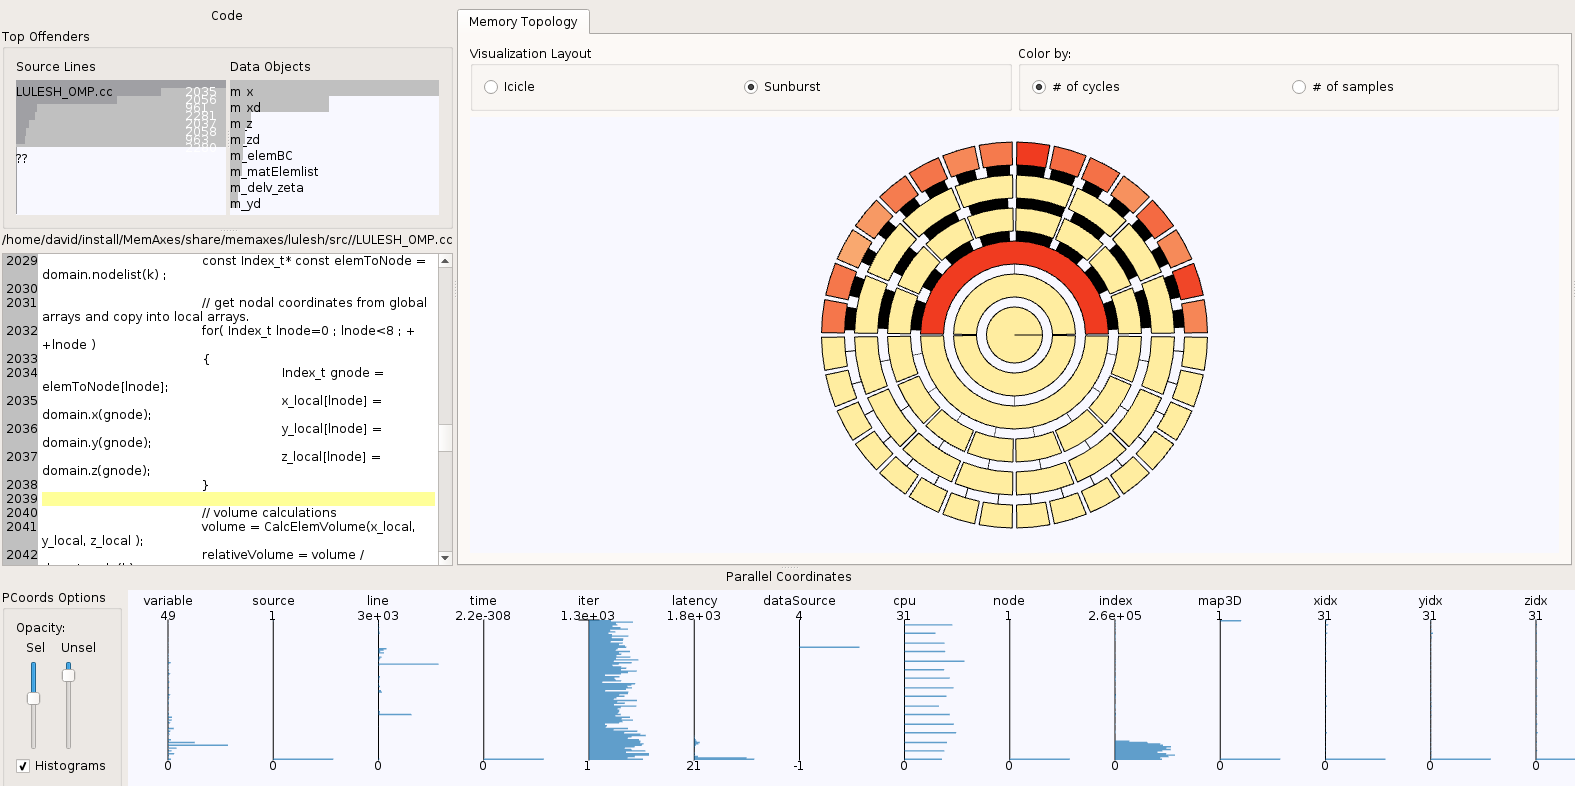
\includegraphics[width=\linewidth]{memAxes.png}
    \caption{Screenshot from MemAxes on the example data trace provided with the
    tool.}
    \label{fig:memaxes}
\end{figure}

Finally, \gls{MemAxes}~\cite{Gimenez14Dissecting} uses memory samples (collected via \gls{PEBS}) and provide a unified view, showed by \fig{memaxes}, that correlate them with the \gls{NUMA} architecture and both code and data structures.
Moreover Husain et al.~\cite{Husain15Relating} have recently added a layer to \gls{MemAxes} that enable to trace simulations and visualize the performance data directly on the simulated objects.
Still, this visualization does not show sharing pattern or access patterns, it only helps identifying the lines of code and data structures responsible for the bad performances.

\section{Conclusions}
\label{sec:mem-cncl}

The memory subsystems have became more and more complex over the last few decades.
As a result, the way a program allocate and access its memory have a significant impact on the performances.
In the end a developer looking for performances must consider the memory access pattern of its application.
Therefore a tool able to collect memory trace and to display access and sharing pattern would be useful for performance optimization.

Most existing memory trace collection tools consider the memory as a monolithic entity and only provides global information such as the bandwidth.
Some tools provides more detailed memory traces.
Still they rely either on  hardware based sampling in which case the resulting trace only shows a small subset of the memory, or on hardware modifications and are thus not usable by real life developers.

When it comes to visualizing these traces, many techniques were developed to identify precisely in the code and data structures where performances are suboptimal.
Yet, most of the existing tools are not able to show memory pattern from any kind.
A few advanced tool allow to see the number of accesses per data structures and per threads or the number of remote accesses per pages.
Still this is not enough information to understand precisely sharing patterns or memory access patterns.

To conclude we need both to collect precise memory traces and to present them to the user in a comprehensive way that enable identification of sharing and access patterns.
% vim: et si sta lbr  sw=4 ts=4 spelllang=en_us
